\section{Morph-GraphQL: GraphQL Server Generation from Declarative Mappings}
\label{chap6_morphgraphql}
Introduced in 2000, Representational State Transfer (REST) has become the most common manner to provide web services in the last decade. Those web services that conform to the REST principles, known as RESTful web services, use HTTP/S and its operations to make requests to the underlying server, such as GET to retrieve objects, POST to add objects, PUT to modify objects and DELETE to remove objects, among others.

Over the years, the complexity of modern software concept has evolved since the inception of REST. For example, typical mobile applications have to take into account aspects that receive little attention in traditional applications, such as the size of data being exchanged/transmitted and the number of API calls being made. These aspects are relevant to the problem known as \textit{over-fetching} and \textit{under-fetching}~\citep{bryant2017graphql,vogel2017experiences,mukhiya2019graphql}. Over-fetching refers to the situation in which a REST endpoint returns more data than what is required by the developer~\citep{bryant2017graphql,vogel2017experiences,mukhiya2019graphql}. For example, a developer may need some information about the name of a user, so she hits the corresponding endpoint (\texttt{/user}). However, the endpoint may return information that is not needed by the client, such as birth date and address. The opposite also raises a problem, which is having the REST endpoint provide less data than required. Such a case is called under-fetching~\citep{bryant2017graphql,vogel2017experiences,mukhiya2019graphql}. It refers to the situation in which a single REST endpoint does not provide sufficient information requested by the client. For example, in order to obtain the names of all friends of a particular user, typically two endpoints may be needed: the first is the endpoint that returns the identifiers of all the friends (\texttt{/friends}), and the second is the one that returns the details of each of the friends based on the identifier (\texttt{/user}).

In order to ameliorate the aforementioned problems, Facebook proposed the GraphQL query language \citep{graphql}, initially being used internally by the company in 2012. GraphQL was released for public use in 2015 and since then has been adopted by companies from various sectors such as technology (GitHub), entertainment (Netflix), finance (PayPal), travel (KLM), among others. 

Two main components of a GraphQL server are \textbf{schema} and \textbf{resolvers}.
The GraphQL schema specifies the type of an object together with the fields that can be queried. GraphQL resolvers are data extraction functions responsible for accessing the underlying datasets. These functions are written by software engineers using a  specific programming language and, are then used by GraphQL engines, which translate GraphQL queries to the corresponding underlying query language of the sources (e.g., SQL). Multiple GraphQL engines support major programming languages (e.g. JavaScript, Python, Java, Golang, Ruby). In addition to the aforementioned frameworks, query planning tools have been developed in order to translate GraphQL queries into other query languages (e.g. dataloader\footnote{\url{https://github.com/facebook/dataloader}}, joinmonster\footnote{\url{https://join-monster.readthedocs.io/en/latest/}}).

Generating a GraphQL server requires expertise from both domain experts and software developers. Typically, the following tasks need to be done: 
\begin{enumerate}
    \item A domain expert would analyse the underlying datasets, propose a unified view schema as a GraphQL schema and how the source datasets would need to be mapped into the GraphQL schema. Note that there is no standard mechanism to represent these mappings. Domain experts may use a spreadsheet, which is not necessarily easy to understand by another domain expert. In the absence of a standard representation, different ways to represent mappings are possible. Some of such spreadsheets represent the relation among source and target concepts in a na\"ive manner using. Others use Excel files with pages, such that each page represents a concept. Others add ids instead of property names.
    It becomes even more messy when there is an operation involved (e.g. source has the name in two properties/columns, ``first-name'' and ``last-name'' while the target has one single attribute to represent both, ``name'').
    \item A software developer would then implement those mappings as GraphQL resolvers, a process that takes significant resources. Given that the complexity of any given source code grows faster than the size of the source code, generating GraphQL resolvers would become more difficult even for a standard-sized dataset which typically contains more than a handful tables and hundreds of properties. This situation might worsen if the underlying dataset evolves, considering that the corresponding resolvers have to be updated as well. GraphQL resolvers may not be easily understood by other developers who were not involved in the initial version, thus bringing the possibility of introducing errors.
\end{enumerate}

In this paper, we propose the exploitation of declarative mapping languages to specify the rules that relate the source datasets and the GraphQL schema. Declarative mapping languages, such as the W3C R2RML~\citep{R2RML} and its extensions, have been used to generate knowledge graphs from existing datasets. The use of declarative mappings is based on the idea that a standard mapping language (or such extensions) would facilitate a better understanding of the relationships between the underlying data source and the exposed GraphQL schema. Furthermore, they also allow for better maintainability as those mappings are independent from any programming language. Our main contribution in this paper is an approach that translates declarative mappings to GraphQL resolvers. We focus on the feasibility of the approach and leave the soundness, completeness, and complexity analysis for future work.

\subsection{The Morph-GraphQL framework}
The Morph-GraphQL framework (Figure \ref{fig:obda2graphql}) proposes the exploitation of the information encoded in declarative mapping rules following a well-known specification (e.g. R2RML and RML) to generate GraphQL servers. A domain expert can create these types of mappings without the need for programming skills. Despite that the creation of mappings might not be easy for domain experts to be created from scratch, there are several tools with easy to use graphical interface that already developed by researchers in the semantic Web community such as RMLEditor~\citep{heyvaert2016rmleditor} or KARMA~\citep{knoblock2015exploiting}. The generated GraphQL servers benefit from the wide range of tools available for GraphQL in order to access data stored in various formats (i.e. RDB, CSV, JSON). The approach consists of the following steps: 1) the generation of the definition of a query to be evaluated by the underlying dataset (e.g. ListEpisodes), 2) the generation of the types in the GraphQL schema and 3) the generation of GraphQL resolvers. 

\begin{figure}[ht]
    \centering
    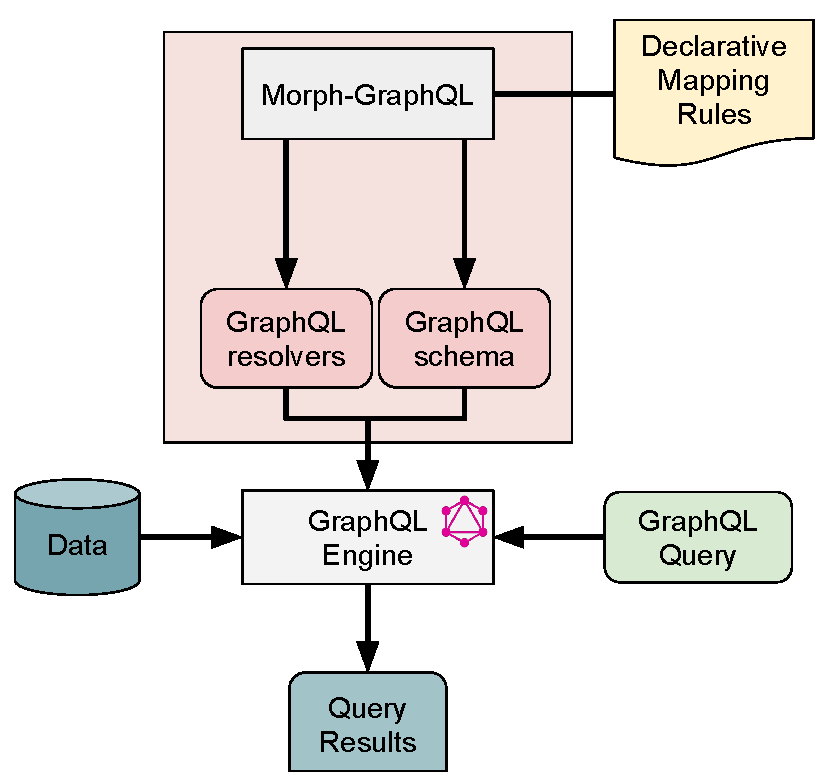
\includegraphics[width=0.8\linewidth]{figures/workflow-morphgraphql.pdf}
    \caption[morph-GraphQL workflow]{\textbf{morph-GraphQL workflow.} morph-GraphQL receives declarative mappings and generates GraphQL servers. These servers, as it is defined in the specification, contain their two main components (i.e. schema and resolvers) that can be used by any GraphQL engine to evaluate queries over the data source.}
    \label{fig:obda2graphql}
\end{figure}



\textbf{Auxiliary Functions}. We present here a set of auxiliary functions that will be used in the functions that generate resolvers.
\begin{itemize}
    \item $getConstant(TermMap)$ takes the constant \texttt{prefix:attr} in the constant-value term map where $TermMap = \texttt{rr:constant "prefix:attr"}$ and retrieves its specific value $attr$.
    \item $getReference(TermMap)$ retrieves the reference \texttt{ref} in the reference-value term map where $TermMap = \texttt{rr:column "ref"}$ or $TermMap = \texttt{rml:reference "ref"}$.
    \item $getTemplate(TermMap)$ retrieves the template \texttt{template} in the template-value term map where $TermMap = \texttt{rr:template "template"}$. In this case, the function retrieves the concatenation between the strings and the references that are part of the template, hence, the implementation of this functions depend of the underlying query system used for retrieving the data. For example, given an SQL database and the term map \texttt{rr:template "ex.com/episode/\{eid\}"} as the inputs, this function returns \texttt{"ex.com/episode/" || eid} or \texttt{CONCAT("ex.com/episode/\{eid\}", eid)}.%, depending on the database system being used.
    \item $getDataType(ObjectMap)$ that given an \texttt{rr:ObjectMap} that contains a \texttt{rr:dataType "xsd:type"} returns the corresponding GraphQL type. For example, $getDataType(rr:dataType ``xsd:string")$ returns \texttt{String}.
    \item $getTypeFromClass(SubjectMap)$ that given an \texttt{rr:SubjectMap} returns the type value based on the \texttt{rr:class} property. For example, $getDataType(rr:class ``foaf:Person")$ returns \texttt{Person}. 
\end{itemize}

\subsubsection{Generating Queries} 
We present a set of translation functions that convert a triples map into the corresponding query to be used in GraphQL resolvers. This set of functions is adapted from the work presented in \citep{chebotko2009semantics}, originally proposed to translate SPARQL queries into SQL queries without the presence of any mappings. For example, given Listing \ref{lst:ex-mappings} as the input, these functions generate the SQL query shown in variable $sql$ in Listing~\ref{lst:EpisodesQueryRoot}.
\begin{itemize}
    \item $\alpha(TriplesMap)$ returns a set of logical sources associated with the triples map $TriplesMap$, which is the logical source associated to the triples map $TriplesMap$ and additionally all the referenced source if $TriplesMap$ contains Referenced Object Maps.
    \item $\beta(TermMap)$ that given a term map $TermMap$ returns the corresponding query expression, that is: 
    \begin{itemize}
        \item $getConstant(TermMap)$ if $TermMap$ is a constant-value map
        \item $getReference(TermMap)$ if $TermMap$ is a reference-value map
        \item $getTemplate(TermMap)$ if $TermMap$ is a template-value map.
    \end{itemize}    
    \item $alias(TermMap)$ generates a unique alias to be used in the query generation.    
    \item $genPR(TriplesMap)$ generates a query expression which projects the relevant query expressions of a triples map $TriplesMap$ (i.e., $\beta$ of Subject Map and all Object Maps) together with their aliases.
    \item $genCond(TriplesMap)$ generates a query expression which is evaluated to true if they match the arguments passed in the resolver functions and additionally the join conditions if $TriplesMap$ contains Referenced Object Maps.
    \item Finally, $trans(TM)$ builds the valid query statement using the results of the previous functions. For example, in the case of an SQL database, \texttt{$trans(TM)$ = "SELECT $genPR(TM)$ FROM $\alpha(TM)$ WHERE $genCond(TM)$"} translates a triples map into the corresponding SQL query.
\end{itemize}

\subsubsection{Generating Schema}
The generation of the Schema for GraphQL is divided into two steps. The first one is focused on the generation of the possible entry points of the server (i.e. the query root) and the second one generates the Types defined for the server. Exploiting the mapping rules as inputs, Morph-GraphQL automatically generates both components.

\subsubsection{Generating Query Root}
First, Morph-GraphQL generates the entry points of the server. Algorithm~\ref{algQueryRoot} shows how this step is executed. Taking as input a mapping document, it iterates over the TriplesMap and extracts the information needed for defining the entry points: the type value extracted from the class property of the subject map and the set of attributes together with the types extracted from the predicate-object maps. Morph-GraphQL is able to generate automatically a set of basic entry points (e.g. ListEpisodes, ListCharacter) that can be filtered by each attribute.
\begin{algorithm}
%\footnotesize
\caption{GenerateQueryRoot(Mapping)}
\label{algQueryRoot}
\begin{algorithmic}
\STATE $queryRoot.init()$
\FORALL{$TriplesMap \leftarrow Mapping$}
    \STATE $typeClass = getTypeFromClass(TriplesMap.getSubjectMap())$
    \STATE $poms = TriplesMap.getPredicateObjectMaps()$
    \FORALL{$pom \leftarrow poms$}
      \STATE $datatype = getDataType(pom.getObjectMap())$
      \STATE $attribute = getConstant(pom.getPredicateMap())$   
      \STATE $attributes.add(attribute,datatype)$
    \ENDFOR
    \STATE $query = createListQuery(typeClass,attributes)$
    \STATE $queryRoot.add(query)$
\ENDFOR
\RETURN $queryRoot$ 
\end{algorithmic}
\end{algorithm}


\subsubsection{Generating Types}
Algorithm \ref{algGenerateSchema} generates a GraphQL type from a Triples Map. It generates a GraphQL type $typeClass$, where $typeClass$ is the class specified in the Subject Map of the Triples Map. The fields of the $typeClass$ are all the mapped predicates in the Predicate Object Maps of the Triples Map. The datatypes of the fields are the results of function $getDataType$, which returns the corresponding GraphQL type from the datatype specified in the Object Maps of the Triples Map. This function is called for each TriplesMap defined in the mapping document.

\begin{algorithm}
%\footnotesize
\caption{GenerateType(TriplesMap)}
\label{algGenerateSchema}
\begin{algorithmic}
\STATE $type.init()$
\STATE $typeClass = getTypeFromClass(TriplesMap.getSubjectMap())$
\STATE $type.add(typeClass)$ 
\STATE $poms = TriplesMap.getPredicateObjectMaps()$
\FORALL{$pom \leftarrow poms$}
  \STATE $datatype = getDataType(pom.getObjectMap())$
  \STATE $attribute = getConstant(pom.getPredicateMap())$
  \STATE $type.add(createAtttribute(attribute, datatype))$
\ENDFOR
\RETURN $type$
\end{algorithmic}
\end{algorithm}


\subsection{Generating Resolvers}
%TBD see Listing \ref{lstGenerateQueryRootResolver}.
%\lstinputlisting[
%frame=single
%, basicstyle=\footnotesize
%, numbers=left
%, label=lstGenerateQueryRootResolver
%, caption=Function generateQueryRootResolver
%, xleftmargin=2em, xrightmargin=2em
%, language=JavaScript
%]{listings/lstGenerateQueryRootResolver.tex}



Algorithm \ref{algGenerateQueryRootNaive} generates a GraphQL resolver from a TriplesMap. Based on the entry points defined in the schema, for each TripleMap, Morph-GraphQL generates the \texttt{list$typeClass$} resolver. First, it defines the function for querying the Type $typeClass$ with the attributes defined in the mapping. Then, the algorithm use the functions defined in section \ref{sec:generateSQL} ($trans$ function) to translate the query to the underlying query language adapting the approach defined in~\citep{chebotko2009semantics}. These two steps use the auxiliary functions $getRereference()$ and $getTemplate()$ in order to obtain the correct references of the data source columns/keys from the mapping rules. Finally, defines the manner how the engines has to executes the query on the underlying database engine and generates the corresponding instances by calling the constructor of Type $typeClass$.

\begin{algorithm}
%\footnotesize
\caption{GenerateResvolver(TriplesMap)}
\label{algGenerateQueryRootNaive}
\begin{algorithmic}[1]
\STATE $resolver.init()$
\STATE $typeClass = getTypeFromClass(TriplesMap.getSubjectMap())$
\STATE $poms = TriplesMap.getPredicateObjectMaps()$
\FORALL{$pom \leftarrow poms$}
  \STATE $attribute = getConstant(pom.getPredicateMap())$
  \STATE $attributes.add(attribute)$
\ENDFOR

\STATE $resolver.add(defineListQueryFunction(typeClass,attributes))$
\STATE $resolver.add(translateQuery(trans(TriplesMap))$
\STATE $resolver.add(execute(query,rdb))$
\STATE $resolver.add(constructResults(attributes,queryResults))$
\RETURN $Resolver$


\end{algorithmic}
\end{algorithm}


\subsection{Morph-GraphQL}
In this section, we present the experimental evaluation of Morph-GraphQL. Our aim is to answer the following questions:
\begin{itemize}
    \item \textbf{RQ1:} Can Morph-GraphQL generate a GraphQL server from declarative mappings that is able to answer the set of queries provided by a GraphQL benchmark?
    \item \textbf{RQ2:} Is there any significant difference between for the queries that can be answered by the generated GraphQL server in terms of response time between GraphQL queries and their equivalent SPARQL queries posed over the RDF dataset generated by the same declarative mappings?
\end{itemize}

We have implemented our framework as an open-source project \textbf{Morph-GraphQL}\footnote{\url{https://github.com/oeg-upm/morph-graphql}}$^,$\footnote{\url{https://doi.org/10.5281/zenodo.3584339}}. In our previous work~\citep{priyatna2019morph} we described the full example of Star Wars generating a GraphQL server based on an R2RML mapping using Morph-GraphQL. Currently, the Morph-GraphQL framework is able to: translate R2RML mappings into a Javascript-based GraphQL server for accessing tabular datasets (CSV files or Relational Databases)\citep{priyatna2019morph}. We use the JoinMonster library\footnote{\url{https://join-monster.readthedocs.io}} to generate efficient SQL queries when joins are needed.

\subsubsection{Link\"{o}ping GraphQL Benchmark} 
Currently, the only GraphQL benchmark available is the Link\"{o}ping GraphQL Benchmark (LinGBM), proposed by Hartig et al.~\citep{hartig2019LinGBM}. This benchmark focuses on exposing read-only GraphQL APIs over a legacy relational database. At the time of writing, the LinGBM benchmark v1.0 sets its context in the domain of e-commerce. It consists of a dataset generator and a set of query templates (a query with placeholder variables to be instantiated). Additionally, guidelines are provided on the mapping between the relational database schema and the GraphQL schema (e.g. Table Offer is mapped to GraphQL type Offer). 

\textbf{Dataset Generator.}
The dataset generator\footnote{\url{https://github.com/LiUGraphQL/LinGBM/wiki/Datasets}} is based on the Berlin SPARQL Benchmark (BSBM)~\citep{bizer2009berlin}. The dataset contains ten tables (e.g.  Vendor, Offer, Producer, Product, and Person, Review) with different join cardinalities (e.g. 1-1, 1-N, M-N).

\textbf{Choke-points and Queries.} 
The benchmark includes a list of \textit{choke-points}, which are challenges that have been identified for answering GraphQL queries. This is done following the design methodology for benchmark development\footnote{\url{http://ldbcouncil.org/blog/choke-point-based-benchmark-design}} introduced by the Linked Data Benchmark Council\footnote{\url{http://ldbcouncil.org/}}. Five classes of choke-points that are proposed are: 
\begin{enumerate}
    \item Choke Points Related to Attribute Retrieval. (1 check-point)
    \item Choke Points Related to Relationship Traversal. (5 choke-points)
    \item Choke Points Related to Ordering and Paging. (3 choke-points)
    \item Choke Points Related to Searching and Filtering. (5 choke-points)
    \item Choke Points Related to Aggregation. (2 choke-points)
\end{enumerate}

These choke-points are covered in the 16 hand-crafted query templates provided by the benchmark. The summarise of the queries, the relation with the proposed choke-points and the support of Morph-GraphQL is show in Table \ref{table:supported-queries}.


\begin{figure}[t]
    \centering
    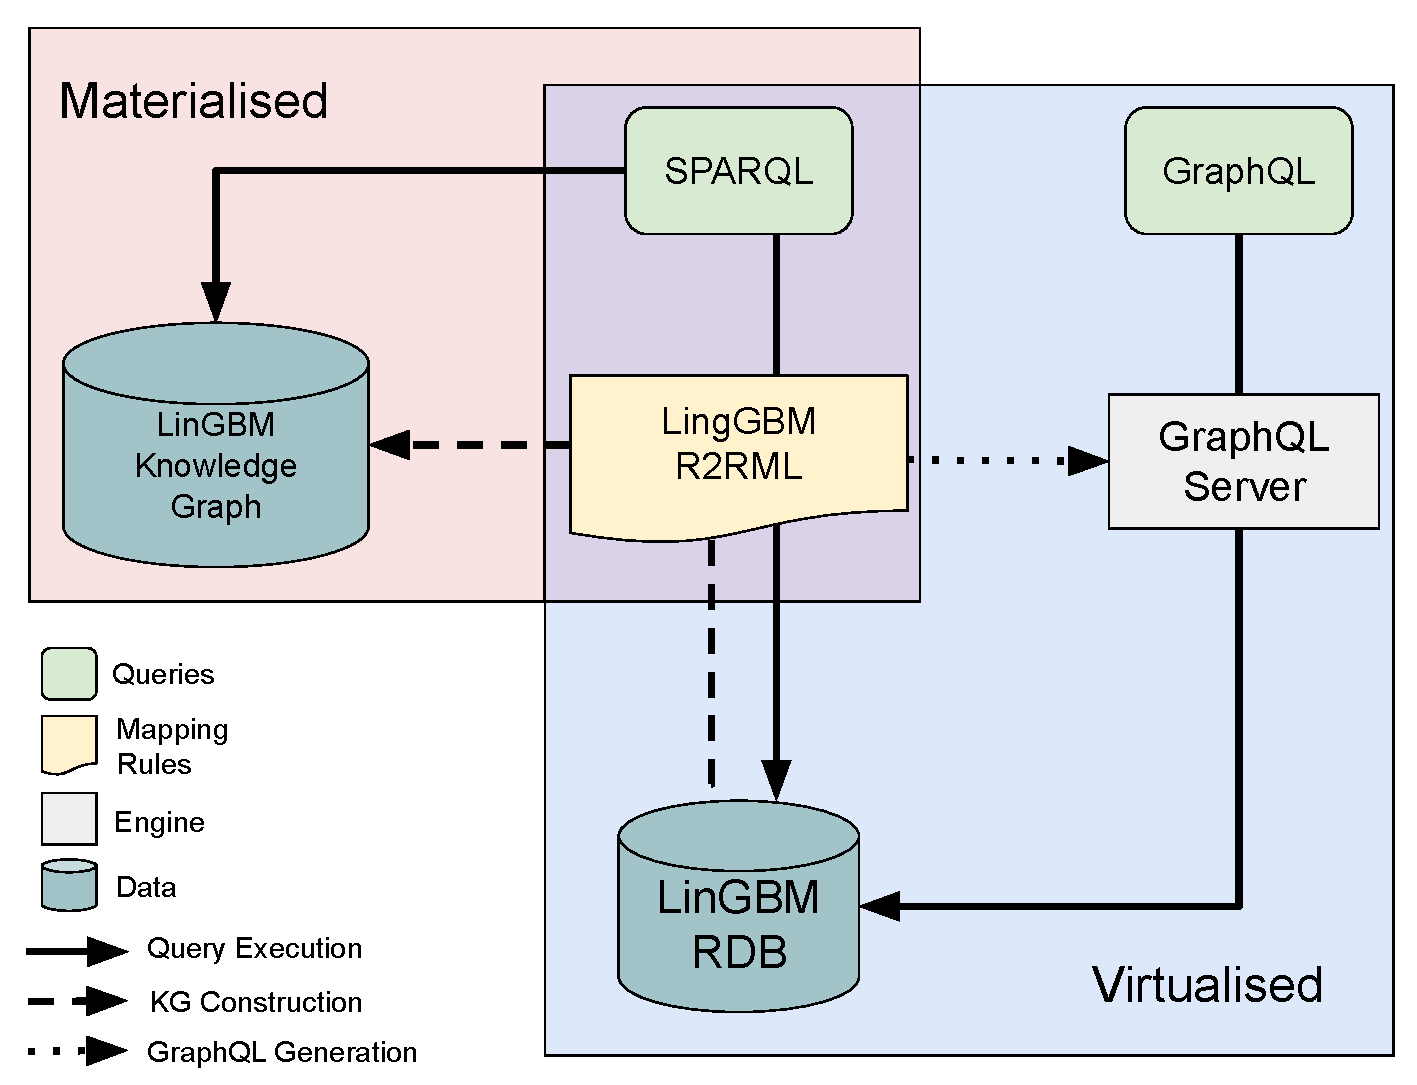
\includegraphics[width=.8\linewidth]{figures/evaluation.pdf}
    \caption[Morph-GraphQL evaluation workflow.]{\textbf{Evaluation Workflow.} We evaluated Morph-GraphQL by comparing its performance over the supported LinGBM queries againts two equivalent Semantic Web approaches. First one is the materialisation of the LinGBM RDB to RDF using R2RML mappings and the second one is the translation from SPARQL-to-SQL using also the the same mapping rules.}
    \label{fig:eval-workflow}
\end{figure}

\subsubsection{Evaluation Setup}
\begin{table}[h!]
 \centering
  \caption[Morph-GraphQL supported LinGBM queries]{Supported Queries in Morph-GraphQL}
 \label{table:supported-queries}
  \begin{tabular}{c | c | c} 
  \toprule
   Query & Choke Points & Morph-GraphQL Support  \\
 \midrule
  Q1 & 1.1, 2.1, 2.2 & Yes   \\ 
  Q2 & 2.1 & Yes  \\
  Q3 & 2.2, 2.3 & Yes   \\
  Q4 & 2.2, 2.3, 2.5 & Yes  \\
  Q5 & 2.1, 2.2, 2.3, 2.4 & Yes  \\ 
  Q6 & 2.2, 2.5 & Yes   \\ 
  Q7 & 2.2, 2.5, 3.2 & No    \\ 
  Q8 & 3.1, 3.3 & No    \\ 
  Q9 & 2.1, 2.2, 3.1, 3.3 & No    \\ 
  Q10 & 1.1, 4.1 & No   \\ 
  Q11 & 2.5, 4.4 & No   \\ 
  Q12 & 2.5, 4.3 & No   \\ 
  Q13 & 2.1, 4.2, 4.3 & No   \\ 
  Q14 & 2.1, 4.2, 4.3, 4.5 & No   \\ 
  Q15 & 5.2 & No   \\ 
  Q16 & 5.1 & No   \\ 
  \bottomrule
  \end{tabular}
 
 \end{table}
We used the LinGBM Data Generator to generate the various sizes of datasets\footnote{The size is defined in terms of number of products in the database (1K means 1 thousand products)} (1K, 2K, 4K, 8K, 16K, 32K, 64K and 128K) and loaded them in the relational database. We created declarative mappings following the mapping guidelines provided in the benchmark. For each query template, we generated 20 queries with different instances generated randomly, as it is the default settings of the benchmark. To measure the performance, we run each query instance 5 times in cold mode, and we calculate the average for each query. We also generated the equivalent SPARQL queries that are to be evaluated over a knowledge graph. The knowledge graph is generated by Morph-RDB \citep{priyatna2014formalisation} from the datasets using the same declarative mappings. 
All the resources used in the evaluation is available online on our GitHub repository\footnote{\url{https://github.com/oeg-upm/morph-graphql/}}.
Figure~\ref{fig:eval-workflow} illustrates the evaluation workflow explained above. The figure shows a materialised and virtualised knowledge graphs. The materialised knowledge graph is the data transformed to RDF and stored into virtuoso ``LinGBM Knowledge Graph'' (a triple store to store knowledge graph data).
The virtualised view does not transform the original datasets to another format (the data is stored in a RDB). It provides access to the underlying datasets via GraphQL. Once a GraphQL query is received, the GraphQL server uses GraphQL engine to translate the query into SQL, which would query the Database ``LinGBM RDB'', get the results, and then the results of the SQL query will be changed into the requested format according to the GraphQL query. We measure the total query execution time for:
\begin{itemize}
    \item GraphQL queries that are translated into SQL queries and evaluated in a relational database instance database. We use Morph-GraphQL v1.0.0 to evaluate these queries.
    \item SPARQL queries that are evaluated over the materialised knowledge graph that is, queries are evaluated using a triple store. We use a Virtuoso v7.2.5.1 instance in this case.
    \item SPARQL queries that are evaluated over the virtual knowledge graph that is, queries are translated into SQL queries and evaluated by Morph-RDB v3.9.15 over the relational database instance. 
\end{itemize}
The experiments were run in an Intel(R) Xeon(R) equipped with a CPU E5-2603 v3 @ 1.60GHz 20 cores, 100G memory with Ubuntu 16.04LTS.

\subsubsection{Results and Discussion}

\begin{table}[]
\centering
\caption[Query execution time of Morph-GraphQL]{Query evaluation performance (time in seconds) over multiple sizes of the LinGBM (the number indicates the scale factor used). Execution time is a lower-is-better metric.}
\label{tab:results}
\resizebox{\textwidth}{!}{%
\begin{tabular}{l|c|c|c|c|c|c|c}
\hline
\multicolumn{1}{c|}{\textbf{Engine/Queries}} & \textbf{Q1} & \textbf{Q2} & \textbf{Q3} & \textbf{Q4} & \textbf{Q5} & \textbf{Q6} & \textbf{\begin{tabular}[c]{@{}c@{}}Geometric\\  Mean\end{tabular}} \\ \hline
\multicolumn{8}{c}{\textbf{LinkGBM 1K}}                              \\ \hline
Morph-GraphQL & 0.103 & 0.146 & 0.005 & 0.118 & 0.237  & 0.079 & 0.075 \\ \hline
Morph-RDB     & 0.168 & 0.081 & 0.201 & 0.221 & 0.296  & 0.089 & 0.159 \\ \hline
Virtuoso      & 0.182 & 0.017 & 0.091 & 0.079 & 1.204  & 0.131 & 0.124 \\ \hline
\multicolumn{8}{c}{\textbf{LinkGBM 2K}}                              \\ \hline
Morph-GraphQL & 0.183 & 0.200 & 0.006 & 0.171 & 0.397  & 0.071 & 0.100   \\ \hline
Morph-RDB     & 0.167 & 0.085 & 0.203 & 0.224 & 0.308  & 0.088 & 0.161 \\ \hline
Virtuoso      & 0.096 & 0.025 & 0.057 & 0.068 & 1.291  & 0.073 & 0.098 \\ \hline
\multicolumn{8}{c}{\textbf{LinkGBM 4K}}                              \\ \hline
Morph-GraphQL & 0.314 & 0.316 & 0.005 & 0.311 & 0.799  & 0.096 & 0.151 \\ \hline
Morph-RDB     & 0.171 & 0.083 & 0.199 & 0.223 & 0.318  & 0.089 & 0.161 \\ \hline
Virtuoso      & 0.109 & 0.035 & 0.059 & 0.078 & 12.293 & 0.101 & 0.167 \\ \hline
\multicolumn{8}{c}{\textbf{LinkGBM 8K}}                              \\ \hline
Morph-GraphQL & 0.597 & 0.644 & 0.004 & 0.625 & 1.363  & 0.096 & 0.228 \\ \hline
Morph-RDB     & 0.178 & 0.080 & 0.196 & 0.225 & 0.323  & 0.090 & 0.162 \\ \hline
Virtuoso      & 0.096 & 0.070 & 0.064 & 0.069 & 2.142  & 0.097 & 0.135 \\ \hline
\multicolumn{8}{c}{\textbf{LinkGBM 16K}}                             \\ \hline
Morph-GraphQL & 1.121 & 1.408 & 0.005 & 1.293 & 2.776  & 0.104 & 0.376 \\ \hline
Morph-RDB     & 0.167 & 0.083 & 0.205 & 0.222 & 0.322  & 0.089 & 0.162 \\ \hline
Virtuoso      & 0.100 & 0.122 & 0.057 & 0.073 & 1.412  & 0.090 & 0.137 \\ \hline
\multicolumn{8}{c}{\textbf{LinkGBM 32K}}                             \\ \hline
Morph-GraphQL & 2.635 & 2.884 & 0.005 & 2.543 & 6.086  & 0.130 & 0.644 \\ \hline
Morph-RDB     & 0.173 & 0.085 & 0.199 & 0.220 & 0.323  & 0.089 & 0.163 \\ \hline
Virtuoso      & 0.108 & 0.274 & 0.069 & 0.085 & 1.591  & 0.122 & 0.179 \\ \hline
\multicolumn{8}{c}{\textbf{LinkGBM 64K}}                             \\ \hline
Morph-GraphQL & 5.157 & 5.940 & 0.005 & 5.114 & 11.065 & 0.147 & 1.050 \\ \hline
Morph-RDB     & 0.177 & 0.085 & 0.199 & 0.224 & 0.325  & 0.090 & 0.164 \\ \hline
Virtuoso      & 0.116 & 0.417 & 0.057 & 0.091 & 1.666  & 0.102 & 0.187 \\ \hline
\multicolumn{8}{c}{\textbf{LinkGBM 128K}}                            \\ \hline
Morph-GraphQL & 8.806 & 9.552 & 0.005 & 8.437 & 22.453 & 0.152 & 1.526 \\ \hline
Morph-RDB     & 0.172 & 0.084 & 0.199 & 0.224 & 0.324  & 0.090 & 0.163 \\ \hline
Virtuoso      & 0.120 & 0.381 & 0.058 & 0.090 & 1.613  & 0.115 & 0.188 \\ \hline
\end{tabular}%
}
\end{table}

In terms of choke-points, Morph-GraphQL supported queries that belong solely to two classes: \textit{attribute retrieval} and \textit{relationship traversal}. Queries which belong to the classes \textit{ordering-and-paging} and \textit{searching-and-filtering} are not supported by Morph-GraphQL. Nonetheless, this can be addressed in a future version of Morph-GraphQL. The last class of chock points addresses \textit{aggregations}, which has not been addressed yet in the GraphQL specification.


We show the results for the different dataset sizes in Table~\ref{tab:results}. We see that for smaller dataset sizes (1K,2K, and 4K), Morph-GraphQL outperforms the others for the majority of the queries. The main reason of these results for smaller dataset sizes is because of the overhead (for translating queries from SPARQL to SQL and optimising the resulting SQL) in Morph-RDB has a negative impact in the total performance of the query execution. Morph-GraphQL needs less time translating the query because it is relatively more simple to translate GraphQL to SQL compared to SPARQL to SQL. In most of the cases for these dataset sizes, Virtuoso needs more time than the other two systems due to the absence of indexes in RDF which has a negative impact depending on the features of the query~\citep{endris2019ontario}. For bigger datasets, SPARQL to SQL optimisations~\citep{priyatna2014formalisation} implemented in Morph-RDB pays off the translation time and gives better impact over the query execution process, outperforming Morph-GraphQL, which hints that the optimisations in the query translation from GraphQL to SQL can still be improved in order to query big datasets (32K, 64K, 128K). When we consider the whole set of queries and calculate the geometric mean of the results, we notice that Morph-GraphQL outperforms the others in some of the dataset sizes because of its fast execution time for the queries Q3 and Q6. Analysing the queries individually, we can observe that for all the engines, Q5 is the most costly one due to the number of nested queries that it consists. 
